\section{Thiết kế Cơ sở dữ liệu và Cơ chế Xác thực}

\subsection{Cấu trúc Lưu trữ Dữ liệu}

\begin{enumerate}
    \item Cơ sở lý thuyết \\
% REMOVED BLANK LINE
    Hệ quản trị CSDL quan hệ (RDBMS) duy trì tính toàn vẹn thông qua các thuộc tính ACID. Lược đồ dữ liệu (Database Schema) tuân thủ dạng chuẩn 3 (3NF) nhằm ngăn ngừa dị thường cập nhật (Update Anomalies). Cơ chế Write-Ahead Logging (WAL) được áp dụng để hỗ trợ xử lý truy vấn đọc/ghi đồng thời (Concurrency) theo dạng phi chặn (Non-blocking).

    \item Triển khai hệ thống \\
% REMOVED BLANK LINE
    Hệ thống sử dụng SQLite3 (RDBMS nhúng) nhằm giảm thiểu độ trễ giao tiếp liên tiến trình (IPC Overhead). Các thiết lập \texttt{PRAGMA journal\_mode=WAL} và \texttt{PRAGMA foreign\_keys=ON} lần lượt hỗ trợ truy xuất đồng thời và thực thi tính toàn vẹn tham chiếu (Referential Integrity). Bảng \ref{tab:db_schema} trình bày chi tiết lược đồ dữ liệu với 5 bảng thực thể.
\end{enumerate}

\renewcommand{\arraystretch}{1.4}
    \begin{longtable}{
        >{\raggedright\arraybackslash}p{2.5cm}
        >{\raggedright\arraybackslash}p{4cm}
        >{\raggedright\arraybackslash}p{7.5cm}
    }
        \caption{Đặc tả các Bảng thực thể trong Cơ sở dữ liệu} \label{tab:db_schema} \\
        \toprule
        \multicolumn{1}{c}{\textbf{Tên Bảng}} & \multicolumn{1}{c}{\textbf{Khóa \& Chỉ mục (Index)}} & \multicolumn{1}{c}{\textbf{Mô tả chi tiết và Vai trò cốt lõi}} \\
        \midrule
        \endfirsthead
        
        \toprule
        \multicolumn{1}{c}{\textbf{Tên Bảng}} & \multicolumn{1}{c}{\textbf{Khóa \& Chỉ mục (Index)}} & \multicolumn{1}{c}{\textbf{Mô tả chi tiết và Vai trò cốt lõi}} \\
        \midrule
        \endhead
        
        \bottomrule
        \endfoot
        
        \bottomrule
        \endlastfoot

        \texttt{Users} & \texttt{PRIMARY KEY (id)} \newline \texttt{UNIQUE (nickname)} & Quản lý thông tin định danh và tham số băm mật khẩu (\texttt{password\_hash}, \texttt{salt}). Hỗ trợ kiểm soát tấn công Brute-force thông qua trường \texttt{failed\_attempts} và \texttt{locked\_until}. \\

        \texttt{Rooms} & \texttt{PRIMARY KEY (id)} \newline \texttt{UNIQUE (room\_name)} & Lưu trữ siêu dữ liệu phòng, bao gồm thông tin xác thực (mật khẩu băm). Cấu trúc khóa ngoại \texttt{creator\_nick} tham chiếu thực thể \texttt{Users} kết hợp ràng buộc \texttt{ON DELETE CASCADE}. \\

        \texttt{RoomBans} & \texttt{PRIMARY KEY (id)} \newline \texttt{idx\_roombans} & Quản lý danh sách cấm (Blacklist) của phòng. Ràng buộc \texttt{UNIQUE(room\_name, nickname)} đảm bảo tính duy nhất của dữ liệu. \\

        \texttt{ChatHistory} & \texttt{PRIMARY KEY (id)} \newline \texttt{idx\_chat\_room\_ts} & Lưu trữ thông điệp mạng. Triển khai chỉ mục liên hợp (Composite Index) trên \texttt{(room, timestamp)} nhằm tối ưu hóa tốc độ truy xuất. \\

        \texttt{AuditLog} & \texttt{PRIMARY KEY (id)} \newline \texttt{idx\_audit\_ts} & Quản lý nhật ký kiểm toán. Áp dụng chuỗi băm (Hash Chain) qua trường \texttt{prev\_hash} để đảm bảo tính toàn vẹn dữ liệu (Tamper-evident). \\
    \end{longtable}

    \begin{figure}[H]
        \centering
        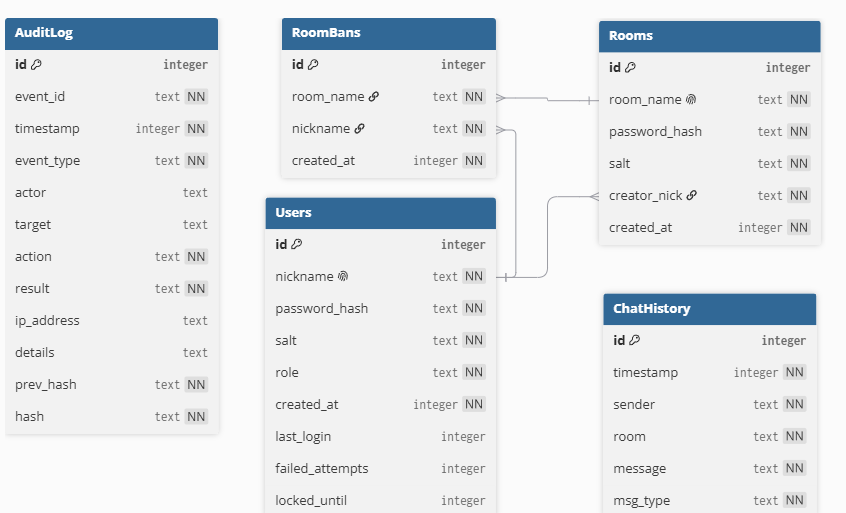
\includegraphics[width=1.0\textwidth]{Hinhve/hinh_2.2.png}

        \caption[Sơ đồ Thực thể Liên kết của hệ thống CSDL]{Sơ đồ Thực thể Liên kết (ERD) của hệ thống CSDL}
        \label{fig:erd_diagram}
    \end{figure}
    



\subsection[Luồng Xác thực và Quản lý Phiên]{Luồng Xác thực và Quản lý Phiên (AuthManager)}

\begin{enumerate}
    \item Cơ sở lý thuyết \\
% REMOVED BLANK LINE
    Kỹ thuật dẫn xuất khóa (Key Stretching) sử dụng hàm PBKDF2 kết hợp chuỗi muối (Salt) nhằm giảm thiểu rủi ro từ tấn công Brute-force và Rainbow Tables. Cơ chế quản lý phiên phi trạng thái (Stateless Session) tích hợp cấu trúc chữ ký mật mã (JWT) và mã xác thực HMAC hỗ trợ giảm tải truy xuất Disk I/O, đồng thời duy trì tính toàn vẹn dữ liệu (Tamper-proof) độc lập với bộ nhớ trạng thái hệ thống.

    \item Triển khai hệ thống \\
% REMOVED BLANK LINE
    Phân hệ \texttt{AuthManager} và \texttt{SessionToken} thực thi quy trình xác thực theo 4 công đoạn:
    
    \begin{itemize}[label={-}]
        \item Khởi tạo định danh: Ứng dụng hàm \texttt{SHA256Hash::pbkdf2()} kết hợp tham số \texttt{salt} để băm mật khẩu. Quá trình đối chiếu mã băm trong pha đăng nhập sử dụng hàm \texttt{CRYPTO\_memcmp()} nhằm hạn chế lỗ hổng phân tích thời gian (Timing Attack).
        \item Cấp phát Token: Module \texttt{SessionToken} đóng gói tập dữ liệu Claims (\texttt{sub}, \texttt{role}, \texttt{exp}, \texttt{jti}) và khởi tạo chữ ký HMAC-SHA256 tuân thủ mô hình phi trạng thái.
        \item Khôi phục kết nối: Gói tin \texttt{MSG\_RECONNECT} chứa Token được xác minh qua chữ ký HMAC trực tiếp trên bộ nhớ chính (RAM), thay thế quy trình truy vấn Cơ sở dữ liệu.
        \item Thu hồi và kiểm soát: Hàm \texttt{SessionToken::revoke()} bổ sung định danh \texttt{jti} vào cấu trúc danh sách đen trong bộ nhớ (In-memory Blacklist) nhằm loại trừ nguy cơ tấn công phát lại (Replay Attack). Phân hệ \texttt{AuthManager} giám sát tần suất đăng nhập sai để kiểm soát tấn công Brute-force.
    \end{itemize}
\end{enumerate}

\begin{figure}[H]
    \centering
    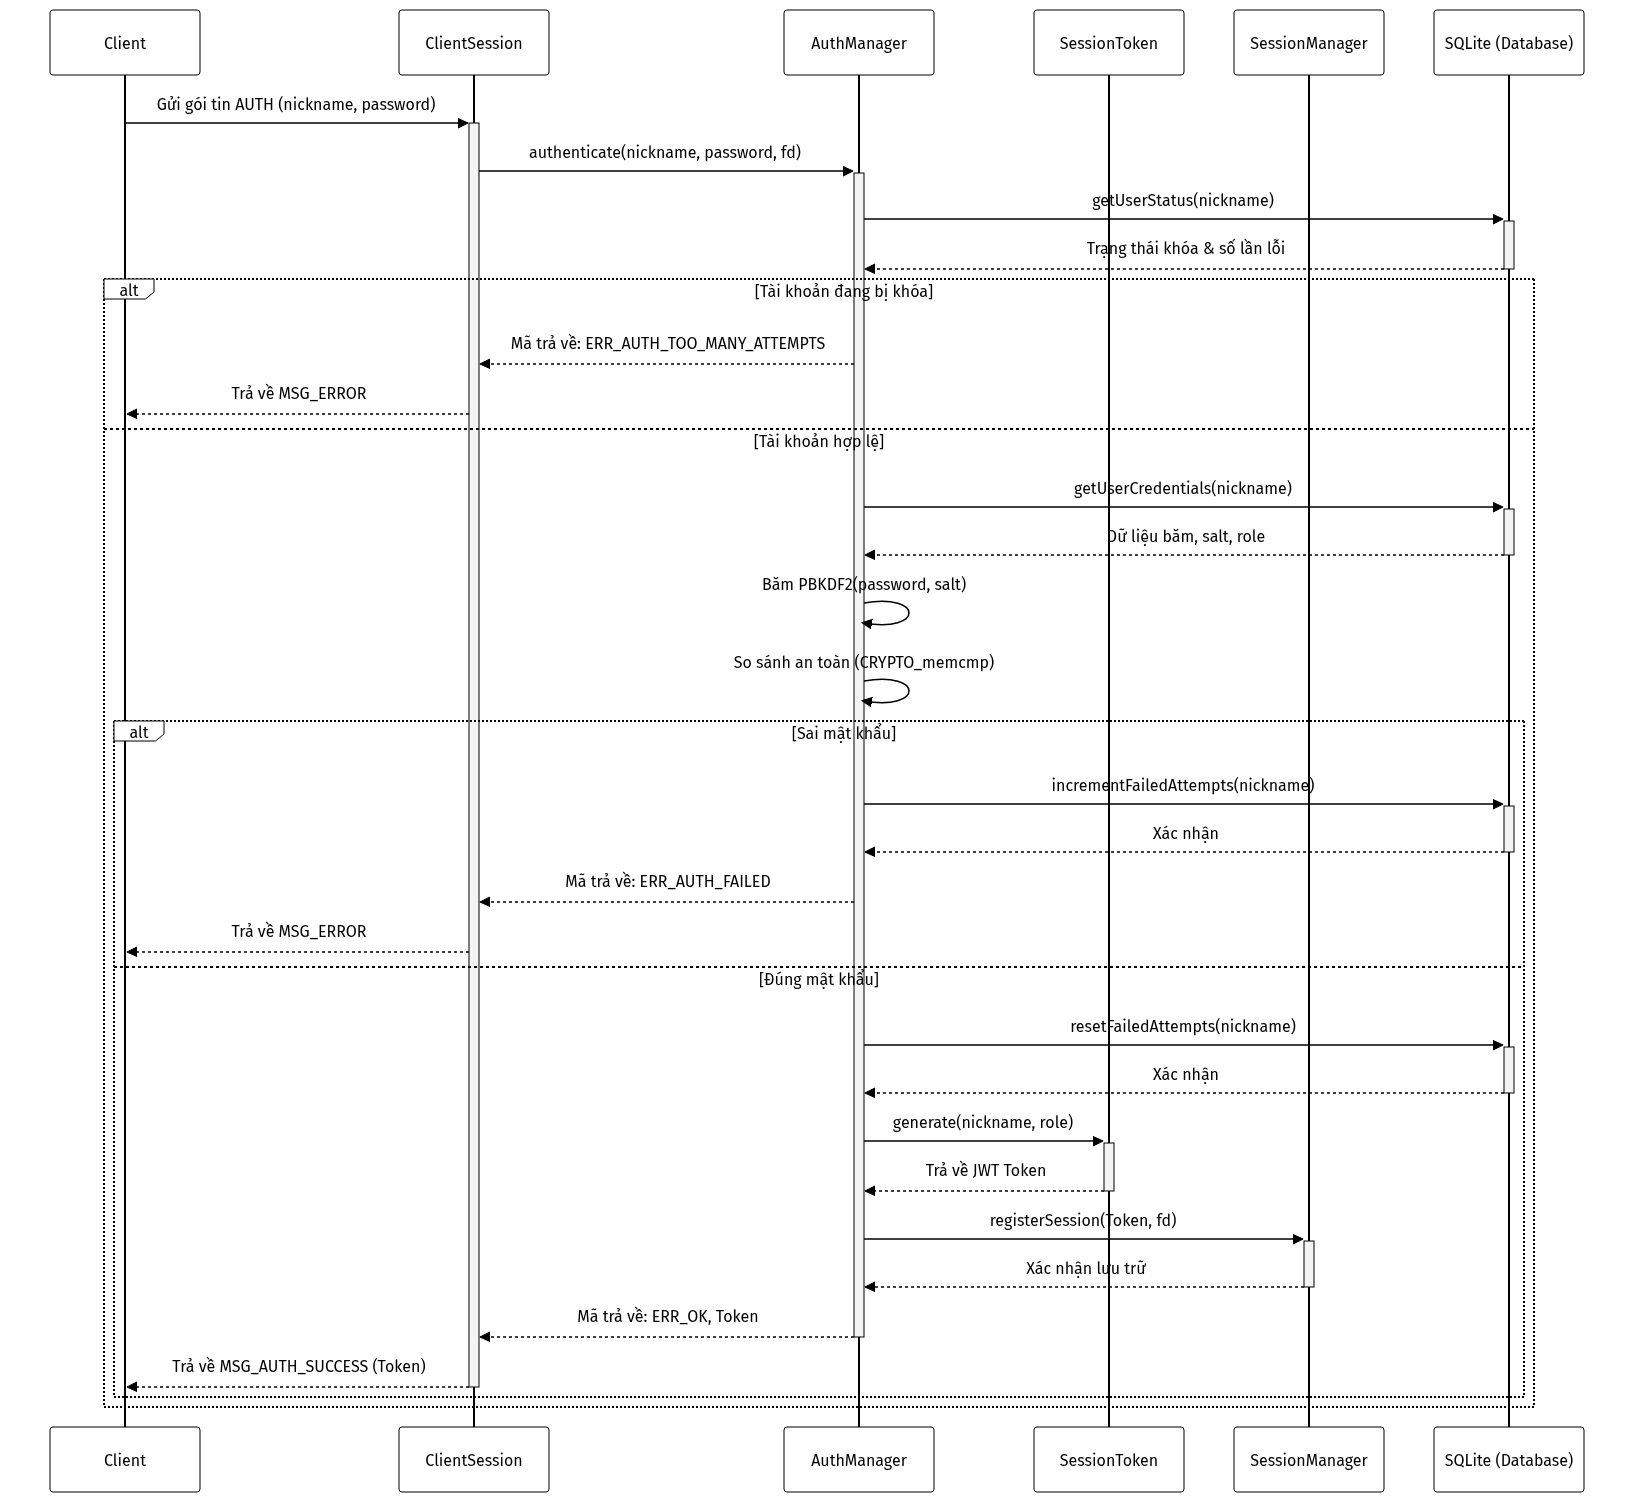
\includegraphics[width=0.9\textwidth]{Hinhve/hinh_2.3.png}
    \caption[Lược đồ Trình tự luồng Xác thực và Khôi phục Phiên]{Lược đồ Trình tự luồng Xác thực và Khôi phục Phiên (Auth \& Reconnect)}
    \label{fig:auth_sequence}
\end{figure}